\section{Additional informations}
\label{ap:age}

The drift velocity used in \ref{fig:age_picture} is given \ref{fig:Reall}.
\begin{figure}[h!]
    \centering
    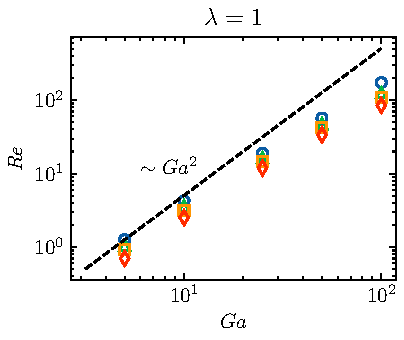
\includegraphics[height = 0.3\textwidth]{image/HOMOGENEOUS_NEW/CA/Re_l_1.pdf}
    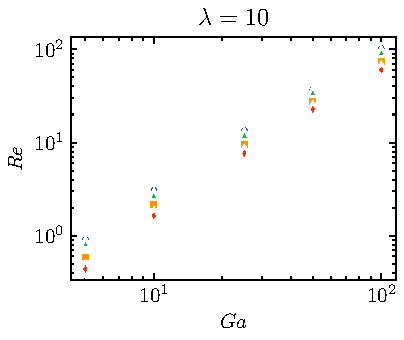
\includegraphics[height = 0.3\textwidth]{image/HOMOGENEOUS_NEW/CA/Re_l_10.pdf}
    \caption{
        Averaged Reynolds number based on the averaged drift velocity, $Re = \rho_fU d /\mu_f$, with $U = |\textbf{u}_p - \textbf{u}_f|$.
        $\textbf{u}_p$ and $\textbf{u}_f$ are the particle and fluid phase volume and time averaged velocity.
    }
    \label{fig:Reall}
\end{figure}


We provide additional age distribution for low \textit{Galileo} number to support the argumentation in the body of the text. 
\begin{figure}[h!]
    \centering
    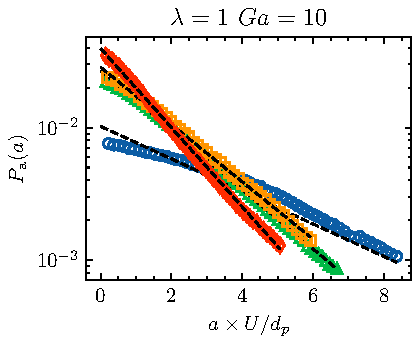
\includegraphics[height = 0.3\textwidth]{image/HOMOGENEOUS_NEW/Dist/Pa_l_1_Ga_10.pdf}
    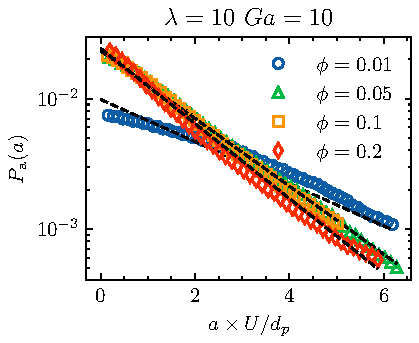
\includegraphics[height = 0.3\textwidth]{image/HOMOGENEOUS_NEW/Dist/Pa_l_10_Ga_10.pdf}
    \caption{(left) Age distribution at $\lambda = 10$ and $Ga = 10$ for : (solid line) $\phi = 0.2$; (dash dotted line) $\phi = 0.1$; (dashed line) $\phi =0.05$; (dotted line) $\phi = 0.01$. 
    (right) Mean dimensionless age in terms of the volume fraction $\phi$ for : 
    ($\bullet$) $Ga=1$; ($\blacktriangle$) $ Ga = 10$; ($\blacksquare$) $Ga = 50$ ($\blacklozenge$) $Ga =100$.
    The age and $\tau_a$ are made dimensionless with $U/d$ where $U$ is the drift-velocity between the dispersed and continuous phase.  }
    \label{fig:age_picture}
\end{figure}